\chapter{\texttt{aRNAque} Appendices}
%\chapter*{\texttt{aRNAque}}


\section{\texttt{aRNAque's GC-content parameters}}
\label{app:b1}
The GC-content is controlled in \texttt{aRNAque} using the mutation parameters $P_C$ and $P_N$. The following table gives the corresponding mutation parameters to the four regimes of GC-content values used for our benchmark. 
\begin{table}[H]
	\centering
	\caption{\textbf{Mutation parameters used in \texttt{aRNAque} to control the GC--content values}.}
	\hspace*{-2.5cm}
	\begin{tabular}{|c|c|c|c|}
		\hline
		GC--content values& $P_C$& $P_N$&\texttt{aRNAque's key } \\
		\hline 
		$0.25$& $\{0.125, 0.125, 0.3, 0.3, 0.075, 0.075\}$ &$\{0.125, 0.125, 0.375, 0.375\}$&GC25 \\
		\hline
		$0.25$& $\{0.25, 0.25, 0.2, 0.2, 0.05, 0.05\}$ &$\{0.25, 0.25, 0.25, 0.5\}$ &GC50\\
		\hline
		$0.75$& $\{0.375, 0.375, 0.1, 0.1, 0.025, 0.025\}$ &$\{0.375, 0.375, 0.125, 0.125\}$&GC75 \\
		\hline
		$1.0$& $\{0.5,0.5,0.0,0.0,0.0,0.0\}$ &$\{0.5,0.5,0.,0.\}$&GC \\
		\hline
	\end{tabular}
	
	\label{tab:my_label}
\end{table}
\section{Benchmark on \texttt{Eterna100} dataset}
\label{app:b2}
For each of the benchmarks on the \texttt{Eterna100} datasets, We ran the first benchmark using the default \texttt{aRNAque}'s parameter configuration. And then, the unsolved structures are sorted out to run a second benchmark with a maximum number of generations set at $5000$. \texttt{aRNAque}'s performance presented in the paper is a combination of all the designed sequences for each realisation.

\section{General EA benchmark parameters }
\label{app:b3}
The same hardware resources and the same computer are used for all the benchmarks listed in the following table. A supercomputer with $40$-Core Intel Xeon E5-2698 v4 at 2.2 GHz and 512 GB of  RAM with a Debian OS. 
\begin{table}[H]
	%\vspace{-1.1cm}
	
	\caption{\textbf{Evolutionary algorithm parameter for each benchmarks}.}
	\hspace{-4cm}
	\begin{tabular}{|p{2.7cm}|p{2cm}|p{2cm}|p{2cm}|p{4.3cm}|p{2cm}|}
		\hline
		Benchmark&Population size&\# of generations (T)& Stopping criterion& Mutation parameter&\# of runs per target \\
		\hline
		PseudoBase++ (\texttt{IPknot})& $100$& $200$& 
		$
		\begin{aligned}
				&t=T \\
				&\max (f) = 0
		\end{aligned}
		$
		& 	
		$
		\begin{aligned}
		&c=1.5 \\
		&P_N=\{0.7,0.1,0.1,.1\}\\
		&P_C=\{0.4, 0.5, 0.1, 0,0,0\}
		\end{aligned}
		$
		&20 \\
		\hline
		PseudoBase++ (\texttt{Hotknots})& $100$& $200$& 
		$
		\begin{aligned}
			&t=T \\
			&\max (f) = 0
		\end{aligned}
		$
		&
		 $
		 \begin{aligned}
		 &c=1.5 \\
		 &P_N=\{0.7,0.1,0.1,.1\}\\
		 &P_C=\{0.4, 0.5, 0.1, 0,0,0\}
		 \end{aligned}
		 $
		 &20\\
		\hline
		PseudoBase++ GC--content (\texttt{IPknot})& $100$& $200$& 
		$
		\begin{aligned}
		&t=T \\
		&\max (f) = 0
		\end{aligned}
		$
		& 
		$
		\begin{aligned}
		&c=1.5 \\
		&P_N=\{0.7,0.1,0.1,.1\}\\
		&P_C=\{0.4, 0.5, 0.1, 0,0,0\}
		\end{aligned}
		$
		&20 \\
		\hline
		Tuning Parameter (\texttt{Binomial,\texttt{IPknot} })& $100$& $200$& 
		$
		\begin{aligned}
		&t=T \\
		&\max (f) = 0
		\end{aligned}
		$
		& 
		$
		\begin{aligned}
		&\mu\in [0,0.2]; c=None \\
		&P_N=\{0.7,0.1,0.1,.1\}\\
		&P_C=\{0.4, 0.5, 0.1, 0,0,0\}
		\end{aligned}
		$
		&20 \\
		\hline
		Tuning Parameter (\texttt{L\'evy}, \texttt{IPknot})& $100$& $200$& 
		$
		\begin{aligned}
		&t=T \\
		&\max (f) = 0
		\end{aligned}
		$
		&
		$
		\begin{aligned}
		&c\in [1,2]; \mu=None \\
		&P_N=\{0.7,0.1,0.1,.1\}\\
		&P_C=\{0.4, 0.5, 0.1, 0,0,0\}
		\end{aligned}
		$ 
		&20 \\
		\hline
		\texttt{Eterna100-V1} (OP, \texttt{RNAfold})& $100$& $5000$& 
		$
		\begin{aligned}
			&t=T \\
			&\max (f) = 0
		\end{aligned}
		$	
		& 
		$
		\begin{aligned}
		&c=7 \\
		&P_N=\{0.7,0.1,0.1,.1\}\\
		&P_C=\{0.4, 0.5, 0.1, 0,0,0\}
		\end{aligned}
		$ 
		&5 \\
		\hline
		\texttt{Eterna100-V1} (L\'evy, \texttt{RNAfold})& $100$& $5000$& 
		$
		\begin{aligned}
		&t=T \\
		&\max (f) = 0
		\end{aligned}
		$
		&
		$
		\begin{aligned}
			&c=1\\
			&P_N=\{0.7,0.1,0.1,0.1\}\\
			&P_C=\{0.4, 0.5, 0.1, 0,0,0\}
		\end{aligned}
		$
		&5 \\
		\hline
		\texttt{Eterna100-V2} (OP, \texttt{RNAfold})& $100$& $5000$& 
		$
		\begin{aligned}
		&t=T \\
		&\max (f) = 0
		\end{aligned}
		$
		& 
		$
		\begin{aligned}
		&c=7 \\
		&P_N=\{0.7,0.1,0.1,.1\}\\
		&P_C=\{0.4, 0.5, 0.1, 0,0,0\}
		\end{aligned}
		$ 
		&5\\
		\hline
		\texttt{Eterna100-V2} (L\'evy, \texttt{RNAfold})& $100$& $5000$& 
		$	
		\begin{aligned}
		&t=T \\
		&\max (f) = 0
		\end{aligned}
		$
		&
		$
		\begin{aligned}
		&c=1.5 \\
		&P_N=\{0.7,0.1,0.1,.1\}\\
		&P_C=\{0.4, 0.5, 0.1, 0,0,0\}
		\end{aligned}
		$ 
		&5 \\
		\hline
	\end{tabular}
	\label{app:tab:EA_parameters}
\end{table}

\section{Other benchmark on \texttt{Eterna100-V1}}
\label{app:b4}
The results on \texttt{Eterna100-V1} presented in the paper are the best of all the benchmarks we have performed. Since our mutation scheme relies on the nucleotide distributions which implicitly control the GC--content of the designed sequences, to obtain our results, we first selected an arbitrary set of pairs $\{P_N, P_C\}$  and benchmark \texttt{aRNAque} on \texttt{Eterna100-V1} for each of them. The success rate measures the fraction of sequences successfully folding into the target structure. Table \ref{app:tab:bp} shows the different parameters we considered and the corresponded input key parameter using the call of \texttt{aRNAque} script.  Summary of the benchmark presented in Table \ref{app:tab:summary} is obtained by launching for each target structure $5$ independent runs, with a population size of $100$ and a maximum number of generations of $5000$. The energy parameter used here was the Turner1999. The dashes in the table mean the benchmarks have not been performed for the parameters.
\begin{table}[t!]
	\caption{\textbf{Different parameters for the base pair distributions}}
	\vspace*{0.5cm}
	\centering
	\begin{tabular}[H]{|c|c|c|}
		\hline 
		\textbf{Key}&\textbf{$P_N = \{p_A, p_G, p_U, p_C\}$ }& \textbf{$P_C = \{p_{GC}, p_{CG}, p_{AU}, p_{UA}, p_{GU},p_{UG}\}$}\\
		\hline 
		$ALL$ & $P_N = \{0.25, 0.25, 0.25, 0.25\}$ & $P_C = \{0.2, 0.2, 0.1, 0.1, 0.2,0.2\}$\\
		\hline
		$GC$& $P_N = \{0.25, 0.25, 0.25, 0.25\}$ & $P_C = \{0.5, 0.5, 0, 0, 0,0\}$\\
		\hline
		$GC_1$& $P_N = \{0.25, 0.65, 0.05, 0.05\}$ & $P_C = \{0.4, 0.5, 0.1, 0, 0,0\}$\\
		\hline
		$GC_2$ & $P_N = \{0.7, 0.1, 0.1, 0.1\}$ & $P_C = \{0.4, 0.5, 0.1, 0, 0,0\}$\\
		\hline
		$GC_3$ & $P_N = \{0.75, 0.1, 0.1, 0.05\}$ & $P_C = \{0.4, 0.5, 0.1, 0, 0,0\}$\\
		\hline
		$GC_4$ & $P_N = \{0.95, 0, 0.05, 0\}$ & $P_C = \{0.4, 0.4, 0.2, 0, 0,0\}$\\
		\hline
		$GC_5$& $P_N = \{0.7, 0.1, 0.1, 0.1\}$ & $P_C = \{0.3, 0.2, 0.2, 0.1, 0.1,0.1\}$\\
		\hline
	\end{tabular}
	\label{app:tab:bp}
\end{table}

\begin{table}[t!]
	\caption{\textbf{Success percentage on \texttt{Eterna100} datasets for each set of mutation parameters}.}
	\centering
	\vspace*{0.5cm}
	\hspace*{-3cm}
	\begin{tabular}[H]{|c|c|p{30mm}|p{25mm}|p{60mm}|}
		\hline 
		\textbf{Tools} &\textbf{BP param}&\textbf{Mutation param}& \textbf{Percentage of success}&\textbf{$\#(Med(gen_{Zipf}) < Med(gen_{op})) $} \newline \textbf{ $\#(Med(gen_{Zipf}) > Med(gen_{op}) )$}\\
		\hline 
		\texttt{aRNAque} & $ALL$& Zipf ($c=1$ )\newline One point & $67\%$ \newline $81\%$ & $7(\# 4)$ \newline $64(\# 4)$\\
		\hline
		\texttt{aRNAque} & $GC$& Zipf ($c=1$ )\newline One point  & $80\%$ \newline $90\%$ &$43(\# 10)$ \newline $30(\# 474)$ \\
		\hline
		\texttt{aRNAque} & $GC_1$& Zipf ($c=1$ ) \newline One point  & $84\%$ \newline $90\%$ &$29(\# 4)$ \newline $33(\# 7)$ \\
		\hline
		\texttt{aRNAque} &  $GC_2$&Zipf ($c=1$ ) \newline One point &  $89\%$ \newline $91\%$ & $61(\# 10)$ \newline $19(\# 1920)$ \\
		\hline
		\texttt{aRNAque} &  $GC_3$ & Zipf ($c=1$ )  \newline One point  &  $88\%$ \newline $--$& $--$ \newline $--$\\
		\hline
		\texttt{aRNAque} & $GC_4$& Zipf ($c=1$ )\newline One point &  $--$ \newline $--$ & $--$ \newline $--$\\
		\hline
		\texttt{aRNAque} &  $GC_5$& Zipf ($c=1$ )  \newline One point &  $82\%$ \newline $83\%$ &$44(\# 9)$ \newline $30(\# 145)$ \\
		\hline
		\textbf{Total}  & -- & Zipf ($c=1$ ) \newline One point  \newline RNAinverse &$\textbf{90\%}$ \newline $\textbf{92\%}$ \newline $\textbf{87\%}$ &\\
		\hline
	\end{tabular}
	\label{app:tab:summary}
\end{table}

\section{Tools patching}
\label{app:b5}
To be able to perform our benchmarks, some slight modifications was made on \texttt{HotKnots} and \texttt{antaRNA}. Details about the modifications are provided in this section.
\begin{itemize}
	\item \texttt{antaRNA}: The change was made at the line 1178 column 7, where the line \textcolor{red}{args = 'HotKnots -m CC -s ' + sequence} was replaced by to \textcolor{green}{args = './HotKnots -m CC -s ' + sequence}. The version of \texttt{antaRNA} we used is v2.0.1, and it can be found on the Github link: 
	\url{https://github.com/RobertKleinkauf/antarna}.
	\item \texttt{HotKnots}: to run \texttt{HotKnots}, we have to move \texttt{aRNAque} to the bin directory. To avoid that, we updated the source code and recompiled a new bin that does not require to move \texttt{aRNAque} to the bin directory of \texttt{HotKnots}. We have uploaded the patched version of \texttt{HotKnots} in a third-part folder in \texttt{aRNAque}'s repository for benchmark reproduction.
	
	\textbf{NB:} The patches do not affect the folding algorithm. It consisted of avoiding the use of relative paths in \texttt{HotKnots}. 
\end{itemize}


\section{\texttt{aRNAque} example calls}
\label{app:b6}
\texttt{aRNAque} computes the RNA inverse folding problem for different classes of structure complexities. 


\noindent For a pseudo-knot free target secondary structure: 

\noindent \rule{12cm}{0.4pt}
\begin{lstlisting}[language=bash, caption={Command line to run \texttt{aRNAque} python script}]
$ python aRNAque.py -t "((....)).((....))"   
			-bp "GC2"
			-sm "NED" 
			-ft "v"
			--job 5
\end{lstlisting}
\rule{12cm}{0.4pt}

\noindent Here, 


\noindent A result to this call could look like this: 

\noindent \rule{12cm}{0.4pt}
\begin{lstlisting}[language=bash, caption={\texttt{aRNAque}'s output results}]
GCUACGGCACCGUCAGG | ((....)).((....)) | -2.8 | 1.0
GGGGGACCACCGGUGGG | ((....)).((....)) | -2.5 | 1.0
GGGCCACCAGCGAAAGC | ((....)).((....)) | -2.2 | 1.0
GGAAAUCCACCGGAAGG | ((....)).((....)) | -1.4 | 1.0
GCAAGAGCGCCGCAAGG | ((....)).((....)) | -1.2 | 1.0
\end{lstlisting}
\noindent \rule{12cm}{0.4pt}

\noindent Where the columns shows respectively the designed sequences, the MFE structures, their free energy and the fitness to the target ( See Equation \ref{eq:fitness})

\section{Lévy flight  vs Local search: designing the structure with the smallest neutral set in the space of all RNA sequences of length  $12$ }
\label{app:b7}
To further illustrate that advantage, we considered the space of all \ac{RNA} sequences of length  $12$ and with only G,C nucleotides. The structures with the lowest neutral set are: 

\begin{enumerate}
	\item $T_1= ((((...)).))$ : only $2$ sequences fold into the secondary structure $T_1$
	\item $T_2= ((.((...))))$ : only $1$ sequence folds into the secondary structure $T_2$
\end{enumerate}

When having a close look at those two structures the base pair density is maximal and there is an unpaired position on both that allows the formation of a budge. 

What that means naively is that any compatible sequence to $T_1$ (or $T_2$) will likely fold into a stem with four or three base pairs( $((((...)))).$ Or $(((....)))..$ ) , and these particular structures have respectively $243$ and $249$ sequences in their neutral sets. 

We claim that, when having such kind of structure ($T_1$ or $T_2$), the levy mutation is of an important role to get out of the huge neutral network of more stable stems. A simple test case was to run \texttt{aRNAque} for a target secondary structure $T_1$.  For both one point and Lévy mutations, the distribution of the number of generations needed to find sequences that fold into $T_1$ for both mutation schemes is plotted in \autoref{fig:target1}. 

\begin{figure}[H]
	
\includegraphics[width=1.0\linewidth]{../res/images/aRNAque/Target1.pdf}
	\caption{\textbf{Distribution of number of generations need to solve the target $T_1$, for both Lévy and Local mutation schemes.}}
	\label{fig:target1}
\end{figure}

\section{Continuous and discontinuous transitions in evolution}
\label{app:b8}
\autoref{fig:contiuity} shows the evolution of the average distance to the tRNA target structure, the intervals of time for which a particular structure is present in the population, and a transition between distinct structures present in the evolutionary path. In Fontana's suggestions, a transition ($S_1 \rightarrow S_2$) between two structures $S_1$ and $S_2$ is considered to be continuous if the structure $S_1$ is 'near' $S_2$. In other terms, $S_2$ is likely to be accessible through the neighbour neutral sequences of $S_1$. 

\graffito{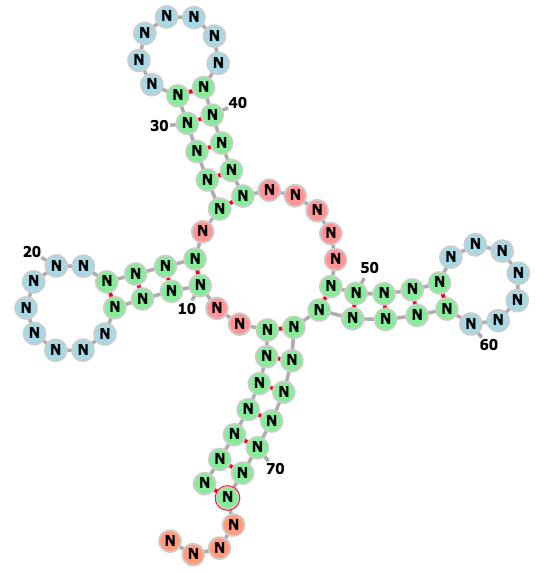
\includegraphics[width=1\linewidth]{../res/images/tRNA_target.png}
	tRNA target secondary structure..}
So if $S_2$ appears in the evolutionary path at time $t$, there exists a time $t'<t$ where $S_2$ was already present in the population. In contrast, the transition is discontinuous otherwise (i.e. the time the structure $S_2$ appears in the evolutionary path exactly at the same time it was present in the population). An example of continuous transition in \autoref{fig:contiuity} is the transition  $18 \rightarrow 10$ whereas the transition $15 \rightarrow 22$ is said to be discontinuous. 


\begin{figure}[t!]
	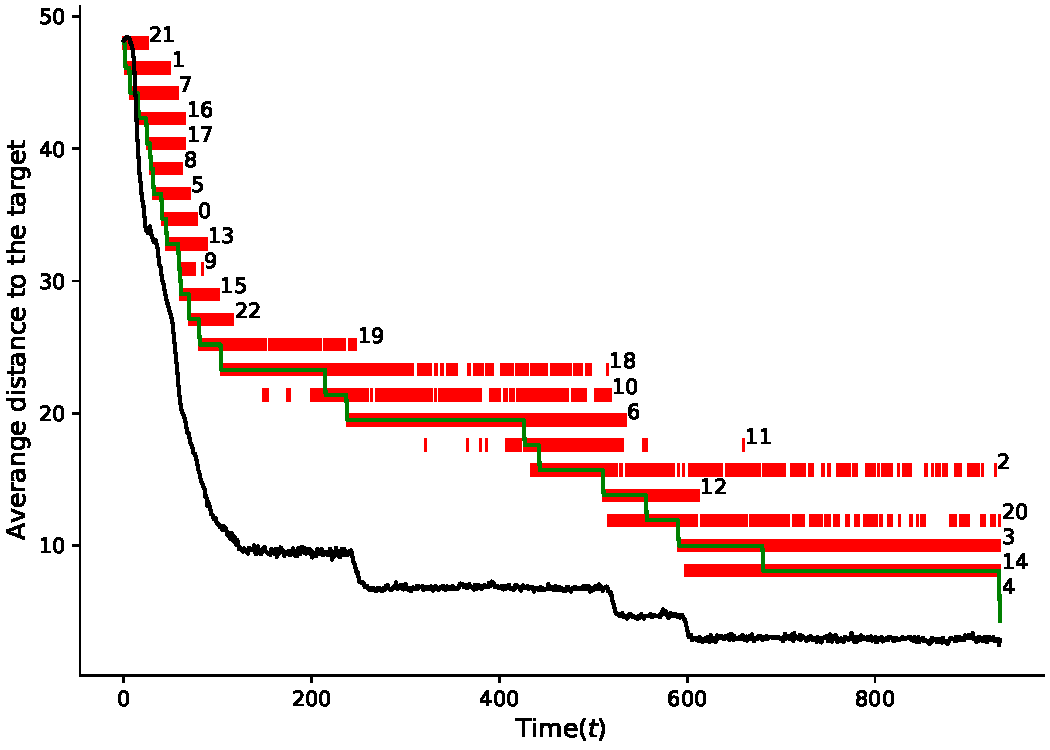
\includegraphics[width=1.0\linewidth]{../res/images/continuity_RNAfold.pdf}
	\caption{\textbf{Simulation of an \ac{RNA} population evolving toward a tRNA (See the figure on the right side) target secondary structure}. The target was reached after $933$ generations (i.e. $\approx 10^5$ replications). The black line shows the average structure distance of the structures in the population to the target structure. The evolutionary history linking the initial structure to the target structure comprises $23$. Each structure is labelled by an integer taken from $0$ to $22$. To each of them corresponds one horizontal line (in red). The top-level corresponds to the initial structure and the bottom the target structure. At each level, a series of red intervals correspond to the periods when the structure was present in the population, and the green curve represents the transition between structures. Only the time axis has a meaning for the red and green curves. }\label{fig:contiuity}
\end{figure}
